% Рисуночки
\section{Конструкторская часть}

\subsection{Требования к программному обеспечению}

\hspace{1.25cm}
На основании введения и поставленных задач сформулированы следующие требования к разрабатываемому программному обеспечению для построения 3D сцен помещений:

\subsubsection{Функциональные требования}
\begin{enumerate}
    \item \textbf{Моделирование помещений и объектов:}
    \begin{itemize}
        \item Возможность добавления базовых 3D объектов: стен, окон, дверей.
        \item Поддержка настройки параметров объектов (длина, ширина, высота, аналогично для отверстия).
        \item Функции перемещения, изменения параметров, вращения и удаления объектов на сцене.
        \item Обеспечение точного размещения объектов с проверкой пересечений и соблюдением заданных границ.
    \end{itemize}
    
    \item \textbf{Управление камерой:}
    \begin{itemize}
        \item Предоставление функций управления камерой для осмотра сцены:
        \begin{itemize}
            \item Вращение вокруг всех трёх осей.
            \item Изменение масштаба для просмотра деталей и общей картины.
        \end{itemize}
    \end{itemize}
    
    \item \textbf{Работа со сценами:}
    \begin{itemize}
        \item Сохранение текущей сцены в файл.
        \item Загрузка ранее сохранённых сцен для продолжения работы.
    \end{itemize}
    
    \item \textbf{Пользовательский интерфейс:}
    \begin{itemize}
        \item Разработка интуитивно понятного интерфейса для работы с объектами и сценой.
        \item Наличие панелей инструментов для выбора объектов, редактирования их параметров и управления камерой.
        \item Поддержка визуализации сцены в реальном времени.
    \end{itemize}
    
    \item \textbf{Производительность:}
    \begin{itemize}
        \item Плавная работа с увеличением количества объектов на сцене.
        \item Оптимизация обработки сцен для предотвращения задержек и рывков при взаимодействии.
    \end{itemize}
    
    \item \textbf{Тестирование:}
    \begin{itemize}
        \item Проверка корректности работы с объектами, сценой и камерой в различных условиях.
        \item Тестирование функций сохранения и загрузки сцен.
    \end{itemize}
\end{enumerate}

\subsubsection{Нефункциональные требования}

\begin{enumerate}
    \item \textbf{Платформенная независимость:}
    \begin{itemize}
        \item Программа должна поддерживать работу на основных операционных системах (Windows, macOS, Linux).
    \end{itemize}
    
    \item \textbf{Простота и удобство использования:}
    \begin{itemize}
        \item Дружелюбный интерфейс, не требующий глубоких технических знаний.
    \end{itemize}
    
    \item \textbf{Надёжность:}
    \begin{itemize}
        \item Минимизация сбоев программы при работе с большими сценами.
        \item Обработка ошибок и предупреждений при неправильных действиях пользователя.
    \end{itemize}
    
    \item \textbf{Расширяемость:}
    \begin{itemize}
        \item Возможность добавления новых типов объектов и функций без значительных изменений в структуре программы.
    \end{itemize}
    
    \item \textbf{Безопасность данных:}
    \begin{itemize}
        \item Сохранение и загрузка файлов без потери данных и повреждения структуры сцены.
    \end{itemize}
\end{enumerate}

\subsubsection{Ожидаемые результаты}

\hspace{1.25cm}
Программное обеспечение должно позволить быстро и эффективно моделировать 3D сцены помещений, обеспечивая интерактивное добавление и редактирование объектов. Оно станет полезным инструментом для анализа, планирования и обучения в области безопасности и оперативного реагирования.


\subsection{Общий алгоритм решения поставленной задачи}

\begin{enumerate}
    \item \textbf{Определение параметров сцены:}
    \begin{itemize}
        \item Установить размеры сцены, на которой будут размещаться объекты.
    \end{itemize}
    
    \item \textbf{Размещение элементов сцены:}
    \begin{itemize}
        \item Разместить необходимые объекты (стены, окна, двери и другие элементы) и определить источники света.
    \end{itemize}
    
    \item \textbf{Визуализация сцены с тенями:}
    \begin{itemize}
        \item На основе текущего положения наблюдателя использовать модифицированный алгоритм, основанный на Z-буфере, для расчёта теней, падающих от объектов сцены.
        \item Выполнить рендеринг сцены с учётом теней и освещения.
    \end{itemize}
\end{enumerate}


\subsection{Алгоритм Z-буфера удаления невидимых линий}
\label{subsection:algo_Zbuff}

\hspace{1.25cm}
Алгоритм Z-буфера удаления невидимых линий на псевдокоде:

\begin{enumerate}
    \item Заполнить буфер кадра фоновым значением интенсивности или цвета.
    
    \item Заполнить Z-буфер минимальным значением глубины \( z \).
    
    \item Преобразовать каждый многоугольник в растровую форму в произвольном порядке.
    
    \item Для каждого пикселя \( (x, y) \) в многоугольнике вычислить его глубину \( z(x, y) \).
    
    \item Сравнить вычисленную глубину \( z(x, y) \) со значением в Z-буфере в этой же позиции \( Z_{\text{буфер}}(x, y) \).
    
    \item \textbf{Запись в буфер кадра:}
    \begin{itemize}
        \item Если \( z(x, y) > Z_{\text{буфер}}(x, y) \), то записать атрибуты многоугольника (интенсивность, цвет и т. п.) в буфер кадра и заменить значение в Z-буфере на \( z(x, y) \).
        \item В противном случае никаких действий не производить.~\cite{roberts}
    \end{itemize}
\end{enumerate}

Блок-схема алгоритма Z-буфера удаления невидимых линий представлена на рисунке~\ref{fig:block_Zbuff}.

\begin{figure}[H]
    \centering
    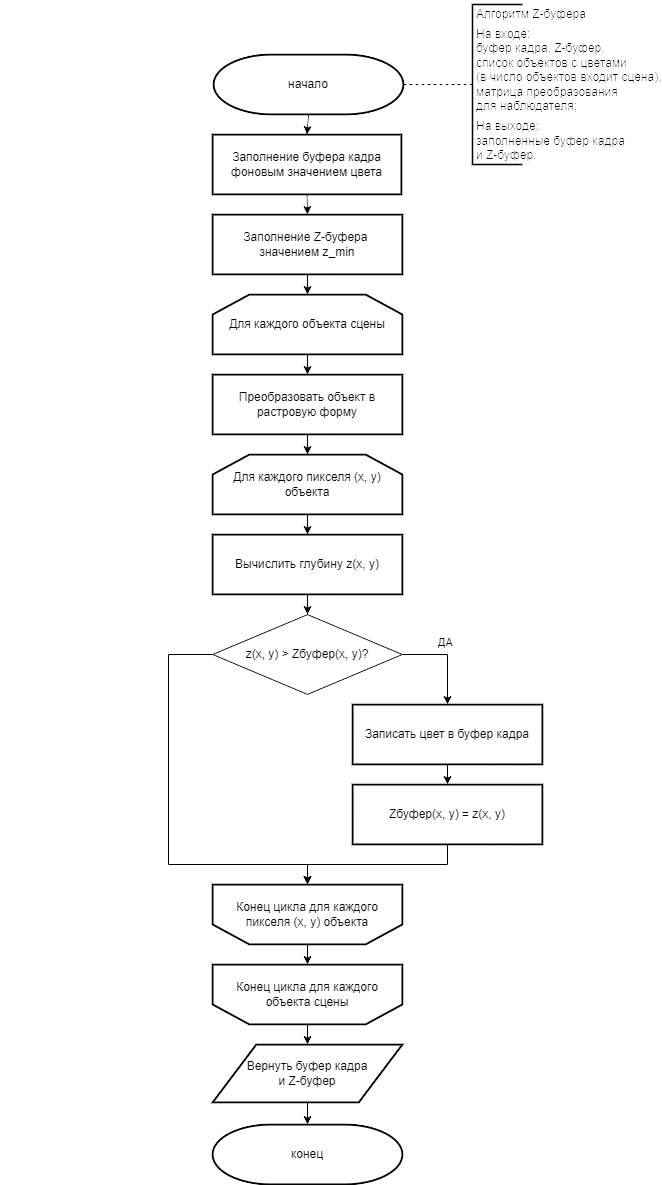
\includegraphics[width=0.8\textwidth]{img/block_1.png}
    \caption{Блок-схема алгоритма Z-буфера удаления невидимых линий.}
    \label{fig:block_Zbuff}
\end{figure}


\subsection{Алгоритм Z-буфера с отрисовкой теней}

\hspace{1.25cm}
Алгоритм Z-буфера с отрисовкой теней на псевдокоде:

\begin{enumerate}
    \item Выполнить расчет Z-буфера для основной сцены:
    \begin{enumerate}
        \item Заполнить буфер кадра фоновым значением интенсивности или цвета.
        \item Заполнить Z-буфер минимальным значением глубины \( z \).
        \item Преобразовать каждый многоугольник в растровую форму в произвольном порядке.
        \item Для каждого пикселя \( (x, y) \) в многоугольнике:
        \begin{itemize}
            \item Вычислить глубину пикселя \( z(x, y) \).
            \item Сравнить \( z(x, y) \) с текущим значением \( Z_{\text{буфер}}(x, y) \).
            \item Если \( z(x, y) > Z_{\text{буфер}}(x, y) \), записать атрибуты пикселя в буфер кадра и обновить \( Z_{\text{буфер}}(x, y) \).
        \end{itemize}
    \end{enumerate}

    \item Выполнить расчет Z-буфера для вида из источника света:
    \begin{enumerate}
        \item Заполнить буфер кадра фоновым значением.
        \item Заполнить Z-буфер минимальным значением глубины \( z \).
        \item Преобразовать каждый многоугольник в растровую форму относительно вида из источника света.
        \item Для каждого пикселя вычислить его глубину \( z(x, y) \) и записать в Z-буфер для создания карты теней.
    \end{enumerate}

    \item Наложить матрицу теней на основную сцену:
    \begin{enumerate}
        \item Для каждого пикселя \( (x, y) \) в Z-буфере основной сцены:
        \begin{itemize}
            \item Извлечь глубину \( z(x, y) \) и преобразовать координаты \( (x, y, z) \) в координаты вида из источника света \( (x', y', z') \).
            \item Если \( x', y' \) находятся в пределах карты теней, сравнить \( z(x, y) \) с глубиной из карты теней \( z_{\text{light}}(x', y') \).
            \item Если \( z(x, y) > z_{\text{light}}(x', y') + \text{EPS} \), уменьшить яркость пикселя или применить цвет тени.
        \end{itemize}
    \end{enumerate}
\end{enumerate}

Блок-схема алгоритма Z-буфера с отрисовкой теней представлена на рисунке~\ref{fig:block_Zbuff_shadow}.

\begin{figure}[H]
    \centering
    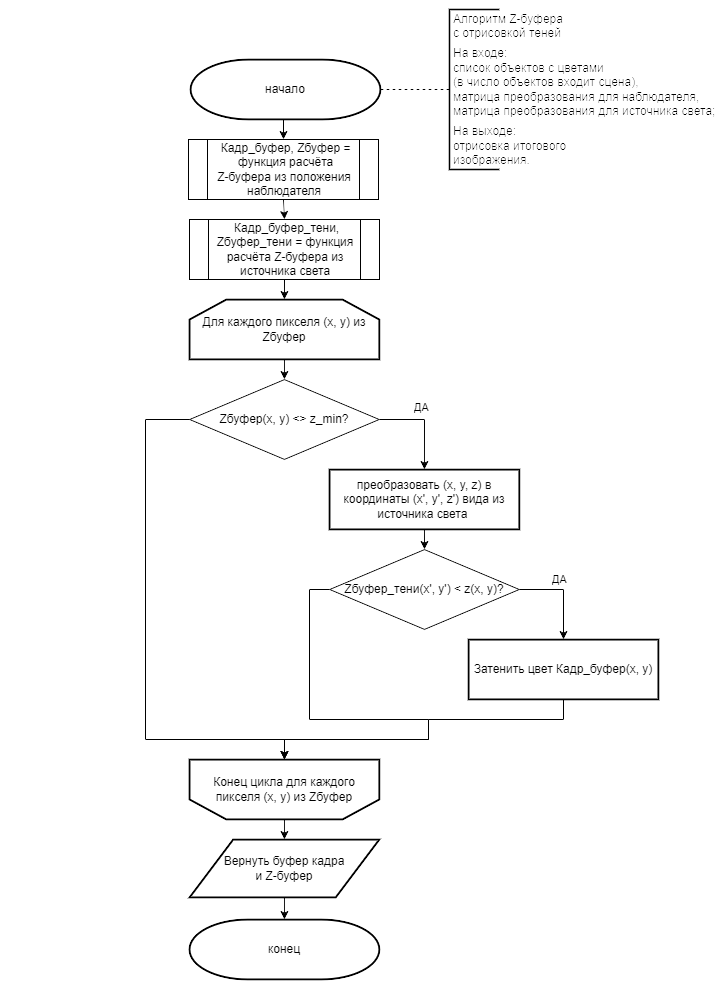
\includegraphics[width=1\textwidth]{img/block_2.png}
    \caption{Блок-схема алгоритма Z-буфера с отрисовкой теней.}
    \label{fig:block_Zbuff_shadow}
\end{figure}



\subsection{Представление объектов в программном обеспечении}

\begin{enumerate}
\item {\bfseries Точка трёхмерного пространства} \\  
   Представлена координатами по осям \(x\), \(y\), \(z\).

\item {\bfseries Стена} \\  
   Задаётся как параллелепипед, параметры которого включают длину, высоту, ширину и координаты начальной точки.

\item {\bfseries Окно} \\  
   Подвид стены, представлено параллелепипедом с параметрами длины, высоты, ширины и расположения (координаты начальной точки).

\item {\bfseries Дверь} \\  
   Аналогично окну, задаётся параллелепипедом с уникальными параметрами длины, высоты, ширины и позиции в пространстве.

\item {\bfseries Сцена} \\  
   Представлена набором плиток (квадратных полигонов), каждая из которых определяется координатами \( (x, y, z) \), где \( z = 0 \) для пола.

\item {\bfseries Камера} \\  
    Описывается матрицей преобразования, включающей параметры положения камеры (координаты) и направления взгляда (углы поворота по осям \(x\), \(y\), \(z\)).

\item {\bfseries Источник света} \\  
   Представлен аналогично камере, с использованием матрицы преобразования, включающей параметры положения источника света (углы поворота по осям \(x\), \(y\), \(z\)).
\end{enumerate}


\subsection{Выводы}

\hspace{1.25cm}
В рамках конструкторской части были сформулированы основные требования к программному обеспечению для моделирования 3D сцен помещений. Также были рассмотрены два ключевых алгоритма рендеринга: алгоритм Z-буфера для удаления невидимых линий и его расширение с отрисовкой теней. Оба алгоритма направлены на создание более реалистичной визуализации сцен с учетом взаимодействия объектов и источника света. Представление объектов в программном обеспечении включает точное описание 3D объектов (стены, окна, двери) и их параметров, а также обработку сцены, камеры и источника света с использованием матрицы преобразования.

Таким образом, работа направлена на создание системы, которая будет эффективно решать задачи моделирования помещений с высокой степенью взаимодействия и визуализации, обеспечивая удобство работы и надежность при взаимодействии с пользователем.


\newpage